\section{Titre}

	\subsection{Sous-titre}
		\begin{frame}
		    \frametitle{\textbf{Titre du slide}}
			\begin{itemize}
				 \item 
				 \item 
			\end{itemize}
			\begin{figure}[h]
				\centering
				
\includegraphics[scale=0.50]{images/tirette/tirette_horizontale.png}
			\end{figure}
		\end{frame}

\subsection{2eme sous-titre}
	\begin{frame}
		\frametitle{\textbf{Titre du 2eme slide}}
		\begin{itemize}
			\item 
			\item 
		\end{itemize}
		\begin{figure}[h]
			\centering
			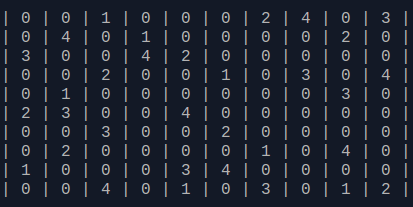
\includegraphics[scale=0.45]{images/boule/boule.png}
		\end{figure}
	\end{frame}